\chapter[Indifference of Description]{The Indifference\\of Description}

\vspace{1em}
\hfill
\begin{minipage}[c]{0.55\textwidth}
\raggedleft
\small\itshape
A man said to the universe:\\
``Sir, I exist!''\\
``However,'' replied the universe,\\
``The fact has not created in me\\
a sense of obligation.''\\[0.5em]
\upshape\footnotesize Stephen Crane (1899)
\end{minipage}%
\hspace{0.5em}
\begin{minipage}[c]{0.12\textwidth}
% \includegraphics[width=\textwidth]{figures/ch10_indifference.png}
\end{minipage}
\vspace{1.5em}

\noindent The framework is built. The thesis is what falls out of it.

The Library contains every computable structure. The universal prior is a measure on it. Your data restrict you to the part of the Library consistent with what you have observed. Within that part you exist at many indices, in many systems, under many possible laws. The measure weights all of it. It singles out none of it: not which index is you, and not which system is real.

This is the book's title.

\section*{Two indifferences}

The first indifference is the one the book has been circling. Among the candidates for \emph{you}, the observers whose memories and sensory state match yours at this moment, the measure has no favorite. Some sit in universes with simple laws, some in baroque ones; some are embedded beings with long lawful histories, some are momentary fluctuations. The measure assigns each a weight, by description length and computational cost. It assigns no one the label \emph{you}. You are a label drawn around a region of the measure. The measure draws no label.

The second indifference is deeper, and it is what this book adds to the first. The measure has no favorite not only among indices but among \emph{systems}. The generator that makes the Library is a single short program: enumerate every program and run it. It does not choose a physics. It runs all of them. Newtonian worlds and relativistic worlds, worlds with three forces and worlds with nine, worlds whose constants are tuned for stars and worlds that collapse in an instant, all of them are in the Library, each at its coordinates, each weighted only by how short a program it takes to specify. No system is marked as the real one. The measure ranks them by simplicity and otherwise has nothing to say.

This is the answer, such as it is, to the question that was the book's reason for being: why this physics, why the particular laws we find, why the Born measure rather than some other weighting of outcomes? The answer is that there is no \emph{why this one}. There is only the measure a finite predictor is forced into, which weights the simple ahead of the complex, and the fact that we find ourselves in a simple system because that is where most of that weight falls. The Born measure, from Chapter 8, is not a separate law handed down with the physics. It is the indexing measure of Chapter 4, the universal prior, restricted to the computable region we inhabit. Ask why the Born rule, and the answer is: because the measure on the Library, seen from inside one of its physical regions, looks like the Born rule.

Here it helps to separate two things the word \emph{simplicity} has been carrying. As a rule for \emph{prediction}, simplicity is not a postulate at all; it is earned. Chapter 5 showed it forced three ways: Kraft makes any other weighting incoherent, dominance makes it optimal, invariance makes it robust to the choice of machine. Ask why an agent should prefer simple explanations and the answer is a theorem, not a preference.

The ontological reading is the other half, and it is where the postulate of Chapter 6 does its work. To read this measure, optimal for \emph{predicting} reality, as also bearing on what \emph{is} real is to stop privileging the one-world cut: not to add that every system exists, but to decline the carving that said only ours does. That declining is the postulate, no cut is privileged, and the mathematics does not force it. It does motivate it. A rule that provably tracks reality better than any computable rival is at least a clue: it suggests reality is the kind of thing this measure is optimal \emph{for}. The clue is not a proof. The best map is not the territory, and ``best predictor of the world'' does not entail ``the world is built like the predictor.'' A reader can take the optimality, decline the postulate, and keep all of Part I. The leap is not arbitrary; it is the natural reading of a very strong result, offered as exactly that.\footnote{The motivation is genuinely vulnerable at one point. Perhaps simplicity predicts well for us only because we are the kind of observer that arises in simple, predictable regions, a selection effect rather than a fact about reality at large. The epistemic result survives the worry: dominance is a theorem about all computable distributions, not about our region in particular. The ontological bridge does not fully survive it, because we would find simplicity ontologically natural either way. That is precisely why it is a bridge and not a proof.}

Granting the postulate, the question bottoms out, though not quite where you might expect. It does not bottom out at ``why is reality simplicity-weighted,'' because there is no privileged measure on reality to explain: the weighting is the finite cutter's, forced by Kraft, and reading it as a property of the world rather than of the predictor is itself one of the cuts the postulate refuses to crown (Chapter 8 made it the open question it is). What does not dissolve is thinner and more stubborn: that there is a space of possibility at all. That is the brute residue, the way the low-entropy past is \emph{Worldlines}' one brute fact, assumed rather than earned. Every \emph{why} above it is answered. It is not answered by anything below.

Figure~\ref{fig:doubled-indifference} puts both indifferences in one picture: the measure ranking systems, and within a system ranking indices, and singling out neither.

\begin{figure}[h]
\centering
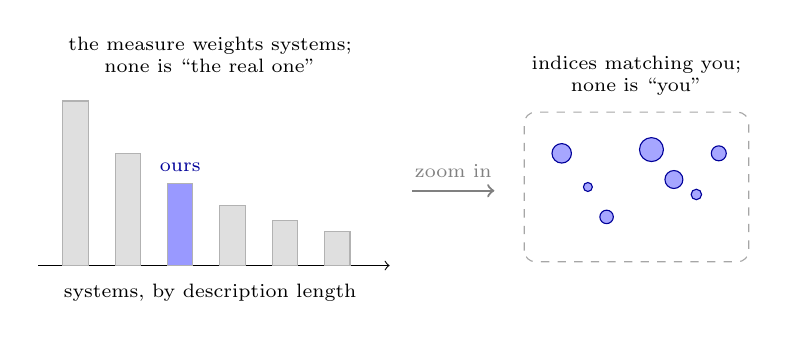
\begin{tikzpicture}[scale=0.95]
  % --- Panel A: the measure over systems ---
  \draw[->] (0,0) -- (4.7,0);
  \node[font=\scriptsize, anchor=north] at (2.3,-0.12) {systems, by description length};
  \foreach \x/\h/\c in {0.5/2.2/gray!25, 1.2/1.5/gray!25, 1.9/1.1/blue!40, 2.6/0.8/gray!25, 3.3/0.6/gray!25, 4.0/0.45/gray!25} {
    \draw[draw=gray!60, fill=\c] (\x-0.17,0) rectangle (\x+0.17,\h);
  }
  \node[font=\scriptsize, blue!60!black, anchor=south] at (1.9,1.12) {ours};
  \node[font=\scriptsize, anchor=south, text width=4.4cm, align=center] at (2.3,2.45) {the measure weights systems;\\none is ``the real one''};

  % --- connector ---
  \draw[->, thick, gray] (5.0,1.0) -- (6.1,1.0);
  \node[font=\scriptsize, gray, anchor=south] at (5.55,1.05) {zoom in};

  % --- Panel B: the measure over indices within ``ours'' ---
  \begin{scope}[shift={(6.5,0)}]
    \draw[rounded corners, dashed, gray!70] (0,0.05) rectangle (3.0,2.05);
    \foreach \x/\y/\r in {0.5/1.5/0.13, 1.1/0.65/0.09, 1.7/1.55/0.16, 2.3/0.95/0.07, 2.6/1.5/0.10, 0.85/1.05/0.06, 2.0/1.15/0.12} {
      \draw[draw=blue!60!black, fill=blue!35] (\x,\y) circle (\r);
    }
    \node[font=\scriptsize, anchor=south, text width=3.0cm, align=center] at (1.5,2.15) {indices matching you;\\none is ``you''};
  \end{scope}
\end{tikzpicture}
\caption{The doubled indifference. The universal prior weights computable systems by simplicity (left): shorter descriptions carry more measure, but no system is singled out as the real one. Within any one system (right), the same measure weights the many indices whose memories and sensory state match yours, and singles out none of them as you. The measure ranks; it does not choose.}
\label{fig:doubled-indifference}
\end{figure}

\section*{The deeper indifference}

A parallel is already familiar from physics. Special relativity tells us that ``now'' is not a fact about the universe but a fact about the observer: two observers moving relative to each other slice spacetime into different presents, and neither slicing is privileged. The natural reading is the \emph{block universe}, a four-dimensional structure in which past, present, and future all exist at their coordinates. Your birth and your death are equally real. The structure contains no preferred moment. This is the indifference of geometry, worked through at length in the companion volume, \textit{Worldlines}; this book does not assume the reader has met it there.\footnote{The two books form a pair. \textit{Worldlines} works through the indifference of geometry from special relativity; this book works through the indifference of description from algorithmic information theory. Either can be read alone. Read together, they make the same kind of argument at two depths of structure.}

The block universe dissolved the unique present: no moment in your worldline is privileged as \emph{now}. The first indifference here dissolves the unique self: no index in your class of patterns is privileged as \emph{you}. The second goes one level further and dissolves the unique world: no system in the Library is privileged as \emph{the} reality. Geometry was indifferent to where you are in your worldline. Description is indifferent to which worldline, in which physics, in which system of laws, you are at all.

There is one more thing the structure does not have, and the last chapter reached it from the other side. It is not overseen. No agent surveys the Library from above; the ladder of minds has no top, and the only thing above all observers is the structure itself, which observes nothing. So this is not the indifference of a mind that has looked and not cared. It is deeper. There is no vantage from which the Library could be cared about, no seer declining to act. The measure singles out no index and no system, and there is no one above it who could single out anything either. Indifference, here, means unwatched.

\section*{What this is and is not}

The indifference is not an erasure. Your experience now is what it is; the moment of reading these words contains what it contains; the structure of your situation is real at the coordinates where you sit. The multiplicity does not undo any of it.

Nor is it annihilation. The pattern that constitutes \emph{you} is instantiated, and each instantiation is real at the coordinates where it occurs. Multiplication does not subtract. If anything it does the opposite: the structure is at many coordinates, each real, each containing whatever it contains.

The label \emph{I} also keeps its meaning. It picks out a region of the measure with certain features in common: a memory structure, a sensory state, a continuity of attention. It does not pick out a metaphysically unique entity, but it does not need to.

Nor does any of this answer \emph{where am I?} That question remains open. The framework permits the question and gives no sharp answer; the literature's attempts (SSA, SIA, the speed prior) all have costs the book chose not to pay. The question is left where it lives, unresolved.

The indifference, then, is a structural fact about the Library and the measure on it. The measure assigns weight to systems and to observer-moments. The weights have no opinion about which system is real or which moment is yours.

\section*{What this does not console}

None of what follows in this book is consolation.

The framework is what it is. The measure is indifferent, over indices and over systems alike. The hellscapes from Chapter 9 are real at their coordinates; the Boltzmann brain hypothesis is open; the framework permits sustained suffering at indices we cannot reach, observers being deceived at coordinates the cut principle forbids us to exclude, versions of you and everyone you love living through anything physically realizable.

The remaining chapters do not argue these away. They walk into what the framework permits and ask: given this, what does it look like to be a finite indexed observer, with a life and people one loves, in a Library that does not single any of it out?

The response that comes is not derived from the mathematics. The mathematics leaves room. The room is what we walk into. Whether what we carry in is enough for what the room holds is not something the book can promise; the last chapter returns to that, and does not close it.

And the mathematics itself might be wrong. The framework takes one postulate, and leans on the quantum reading besides; either could fail. The response we choose does not depend on which way the cosmology turns out. The room is what we walk into either way.

\section*{Where this leaves you}

The thesis is stated. The book's title is on the page.

The next five chapters trace what the indifference does to continuation, death, love, the self, and what to do anyway. The arguments will follow from the framework already in place. The reader who has followed the cascade has all the tools.

The next chapter takes up continuation.
